\subsubsection{ The Next Read gadgets }

The second part of the return gadgets is the {\nextread} gadget. This type of gadget attaches to the last tile of a {\returnpath} gadget,
and (except in the initial value), outputs either an empty {\cread} signal or a {\tt Cross\_Next\_Row} signal.


For each $\inc\in \{ {\tt increment}, {\tt copy} \}$:
\begin{itemize}

    % DIGIT 1
    \item Create
    $\begin{aligned}[t]
        \nextread(& \left\langle {\tt NextRead}, 1,          \inc \right\rangle,
                    \left\langle {\tt Read},     2, \lambda, \inc \right\rangle \;)
    \end{aligned}$\\from the micro-gadget shown in Figure~\ref{fig:next_read_1-or-2_op}.

    \item Create
    $\begin{aligned}[t]
        \nextread(& \left\langle {\tt NextRead}, 1,          \inc, {\tt msr} \right\rangle,
                    \left\langle {\tt Read},     2, \lambda, \inc            \right\rangle \;)
    \end{aligned}$\\from the micro-gadget shown in Figure~\ref{fig:next_read_1_op_msr}.

    \item Create
    $\begin{aligned}[t]
        \nextread(& \left\langle {\tt NextRead}, 1,      \inc, {\tt msr}, {\tt msd} \right\rangle,
                    \left\langle {\tt Cross\_Next\_Row}, \inc                       \right\rangle \;)
    \end{aligned}$\\from the micro-gadget shown in Figure~\ref{fig:next_read_1-or-2_op_msr_msd}.


    % DIGIT 2
    \item Create
    $\begin{aligned}[t]
        \nextread(& \left\langle {\tt NextRead}, 2,          \inc \right\rangle,
                    \left\langle {\tt Read},     3, \lambda, \inc \right\rangle \;)
    \end{aligned}$\\from the micro-gadget shown in Figure~\ref{fig:next_read_1-or-2_op}.

    \item Create
    $\begin{aligned}[t]
        \nextread(& \left\langle {\tt NextRead}, 2,      \inc, {\tt msr}, {\tt msd} \right\rangle,
                    \left\langle {\tt Cross\_Next\_Row}, \inc                       \right\rangle \;)
    \end{aligned}$\\from the micro-gadget shown in Figure~\ref{fig:next_read_1-or-2_op_msr_msd}.


    % DIGIT 3
    \item Create
    $\begin{aligned}[t]
        \nextread(& \left\langle {\tt NextRead}, 3,          \inc \right\rangle,
                    \left\langle {\tt Read},     1, \lambda, \inc \right\rangle \;)
    \end{aligned}$\\from the micro-gadget shown in Figure~\ref{fig:next_read_3_op}.

    \item Create
    $\begin{aligned}[t]
        \nextread(& \left\langle {\tt NextRead}, 3,      \inc, {\tt msr}, {\tt msd} \right\rangle,
                    \left\langle {\tt Cross\_Next\_Row}, \inc \right\rangle \;)
    \end{aligned}$\\from the micro-gadget shown in Figure~\ref{fig:next_read_3_op-or-seed_msr_msd}.
\end{itemize}

\begin{figure}[H]
    \centering
    \subcaptionbox{Digit 1 \& 2 - general\label{fig:next_read_1-or-2_op}}
    {\makebox[0.24\textwidth][c]{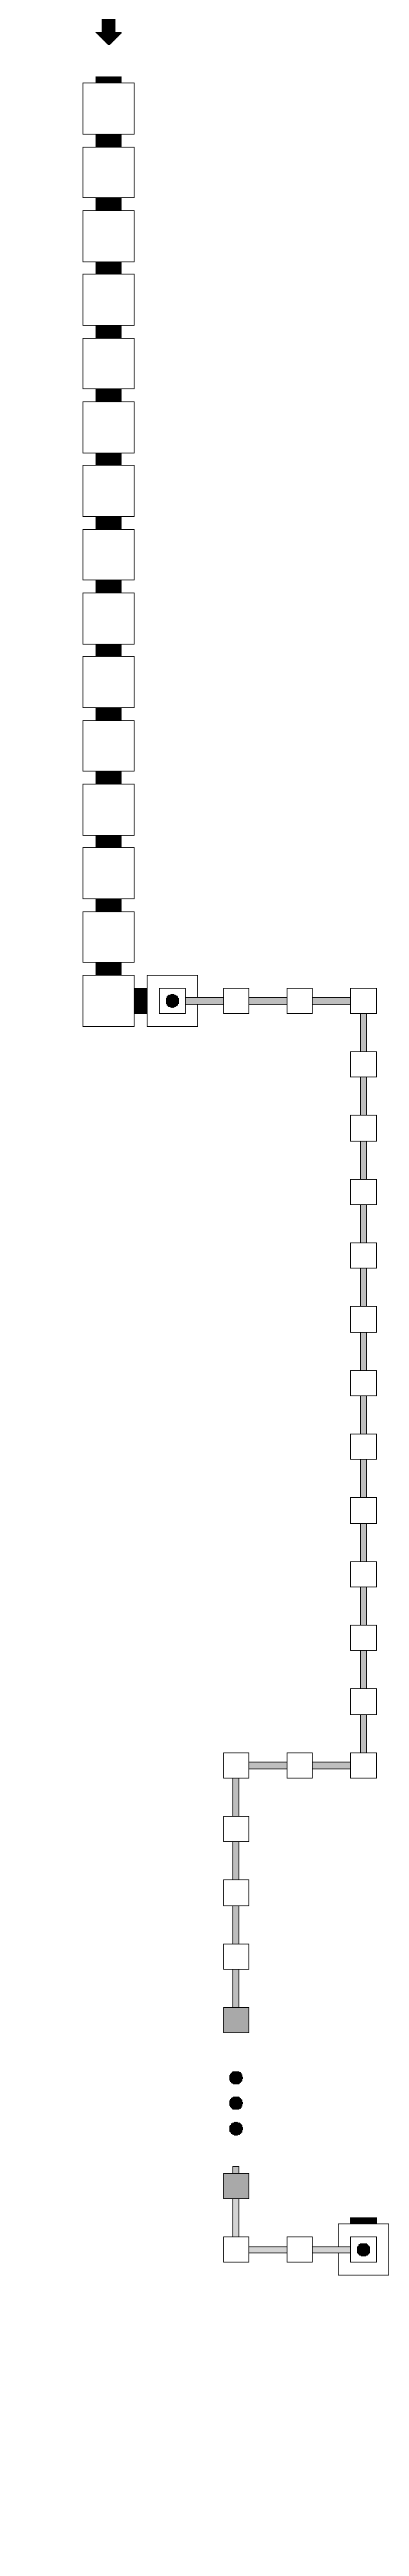
\includegraphics[width=0.45in]{next_read_1-or-2_op}}}%
    ~
    \subcaptionbox{Digit 1 - general\\overview\label{fig:next_read_1_op_overview}}
    {\makebox[0.24\textwidth][c]{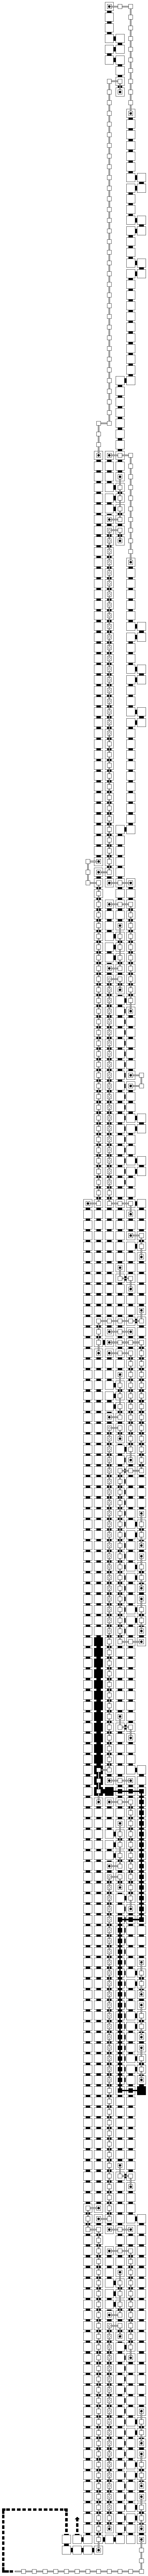
\includegraphics[width=0.45in]{overviews/general/next_read_1_op}}}%
    ~
    \subcaptionbox{Digit 2 - general\\overview\label{fig:next_read_2_op_overview}}
    {\makebox[0.24\textwidth][c]{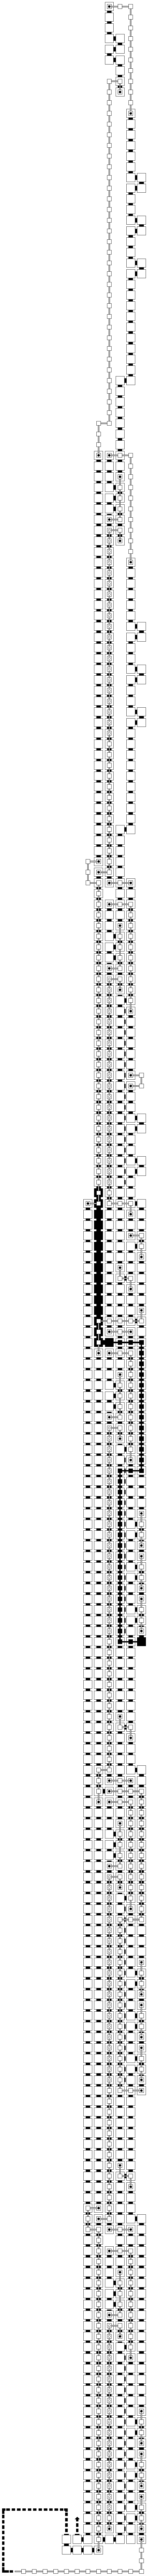
\includegraphics[width=0.45in]{overviews/general/next_read_2_op}}}%
    ~
    \subcaptionbox{Digit 1 - general (seed) overview\label{fig:next_read_1_seed_op_overview}}
    {\makebox[0.24\textwidth][c]{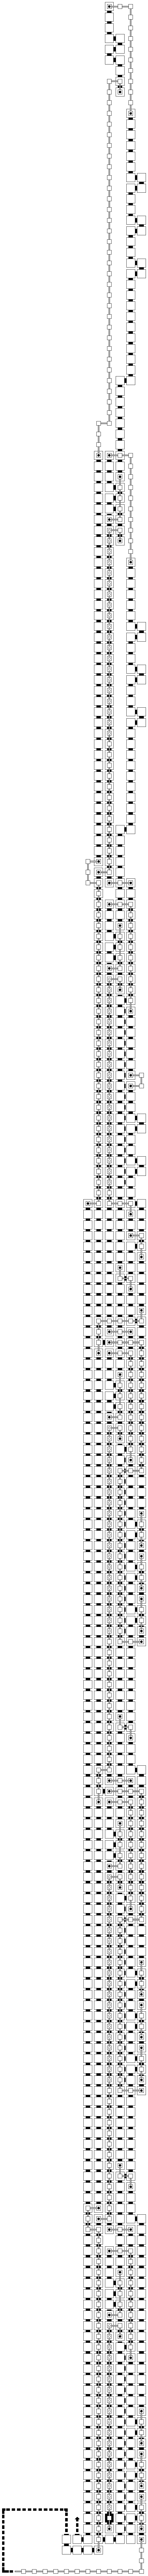
\includegraphics[width=0.45in]{overviews/general/next_read_1_seed_op}}}%
    ~
\end{figure}

\begin{figure}[H]\ContinuedFloat
    \centering
    \subcaptionbox{Digit 2 - seed\label{fig:next_read_2_seed_op}}
    {\makebox[0.24\textwidth][c]{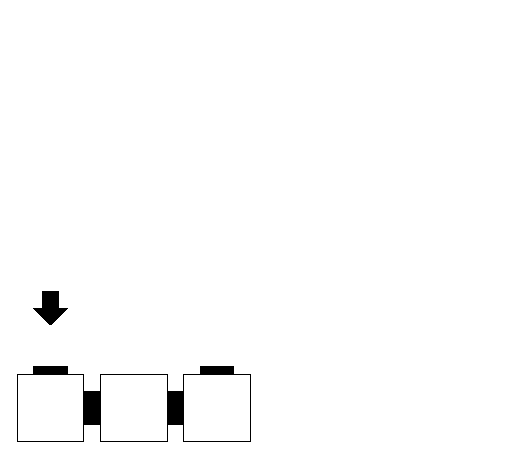
\includegraphics[width=0.45in]{next_read_2_seed}}}%
    ~
    \subcaptionbox{Digit 2 - general\\(seed) overview\label{fig:next_read_2_seed_op_overview}}
    {\makebox[0.24\textwidth][c]{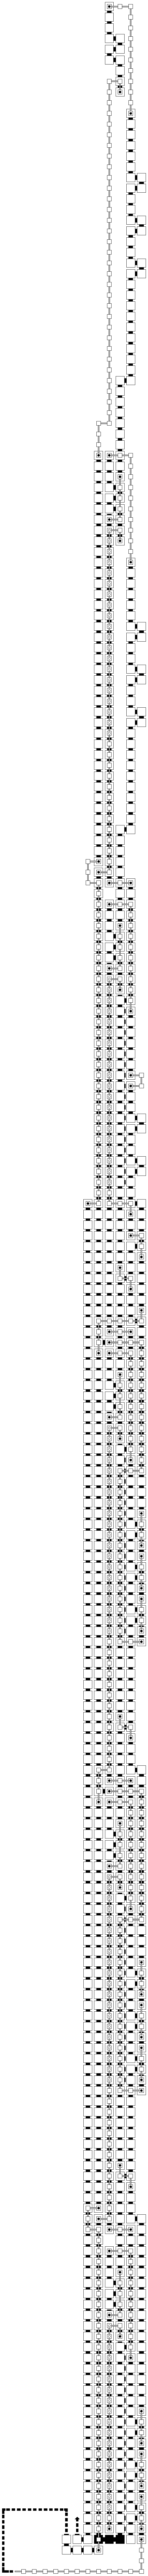
\includegraphics[width=0.45in]{overviews/general/next_read_2_seed_op}}}%
    ~
    \subcaptionbox{Digit 3 - general\label{fig:next_read_3_op}}
    {\makebox[0.24\textwidth][c]{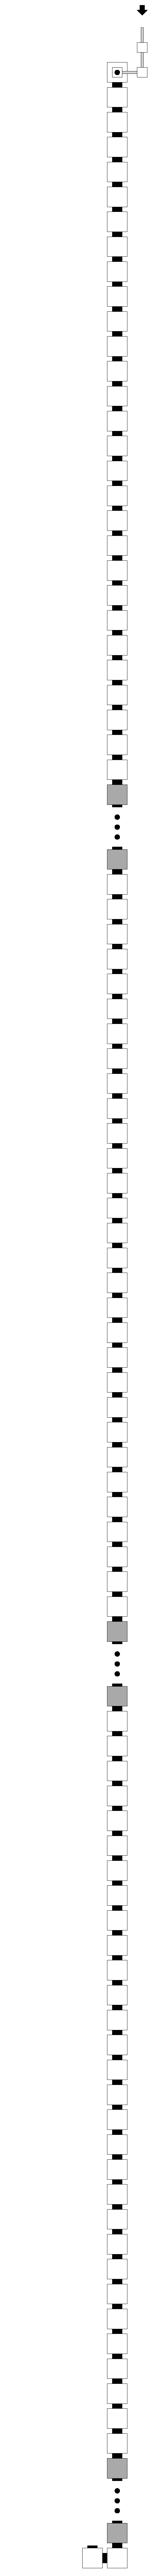
\includegraphics[width=0.45in]{next_read_3_op}}}%
    ~
    \subcaptionbox{Digit 3 - general\\ overview\label{fig:next_read_3_op_overview}}
    {\makebox[0.24\textwidth][c]{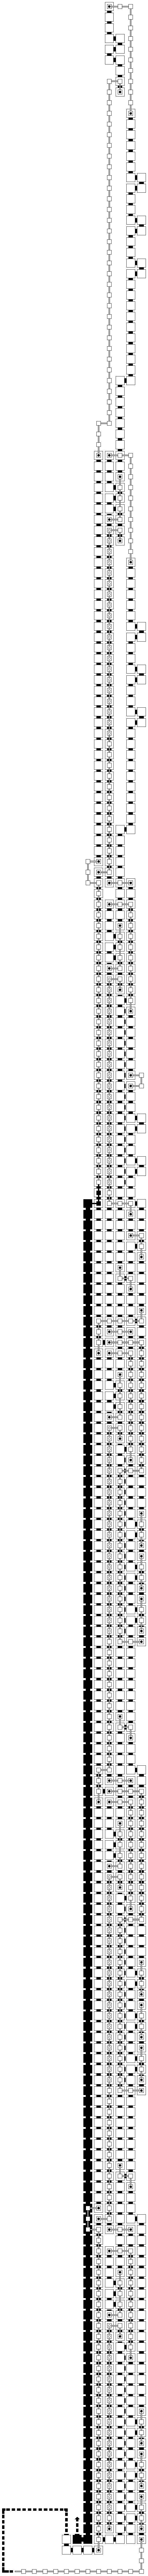
\includegraphics[width=0.45in]{overviews/general/next_read_3_op}}}%
    ~
\end{figure}

\begin{figure}[H]\ContinuedFloat
    \centering
    \subcaptionbox{Digit 3 - seed\label{fig:next_read_3_seed_op}}
    {\makebox[0.24\textwidth][c]{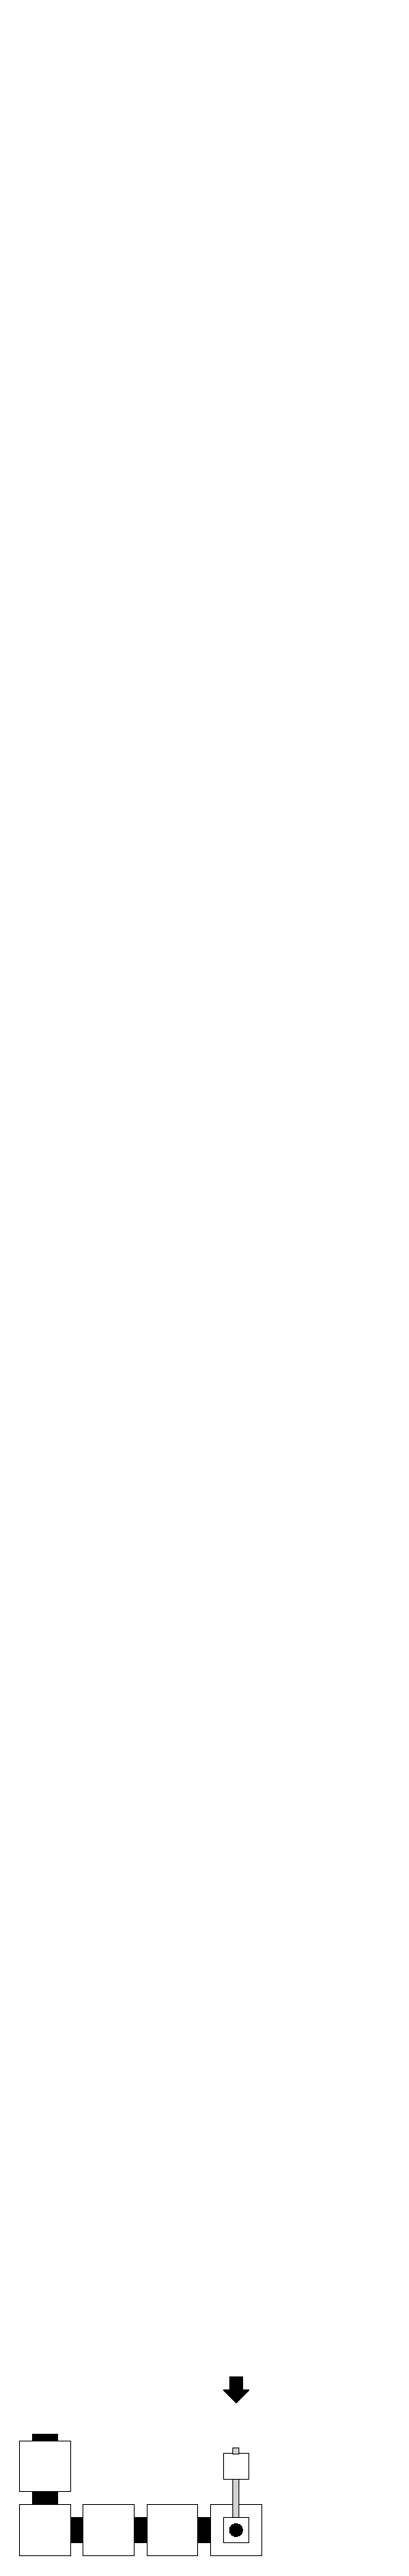
\includegraphics[width=0.45in]{next_read_3_seed}}}%
    ~
    \subcaptionbox{Digit 3 - general\\(seed) overview\label{fig:next_read_3_seed_op_overview}}
    {\makebox[0.24\textwidth][c]{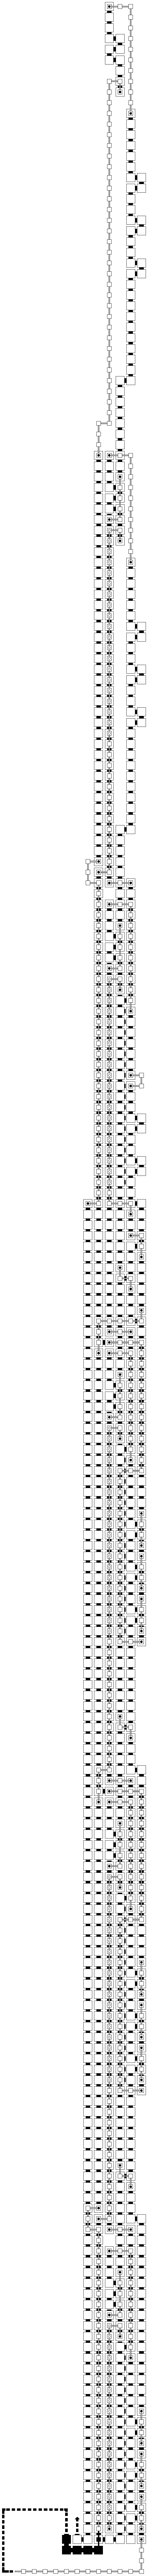
\includegraphics[width=0.45in]{overviews/general/next_read_3_seed_op}}}%
    ~
    \subcaptionbox{Digit 1 - case 1, Digit 2 - case 2\label{fig:next_read_1-or-2_op_msr_msd}}
    {\makebox[0.24\textwidth][c]{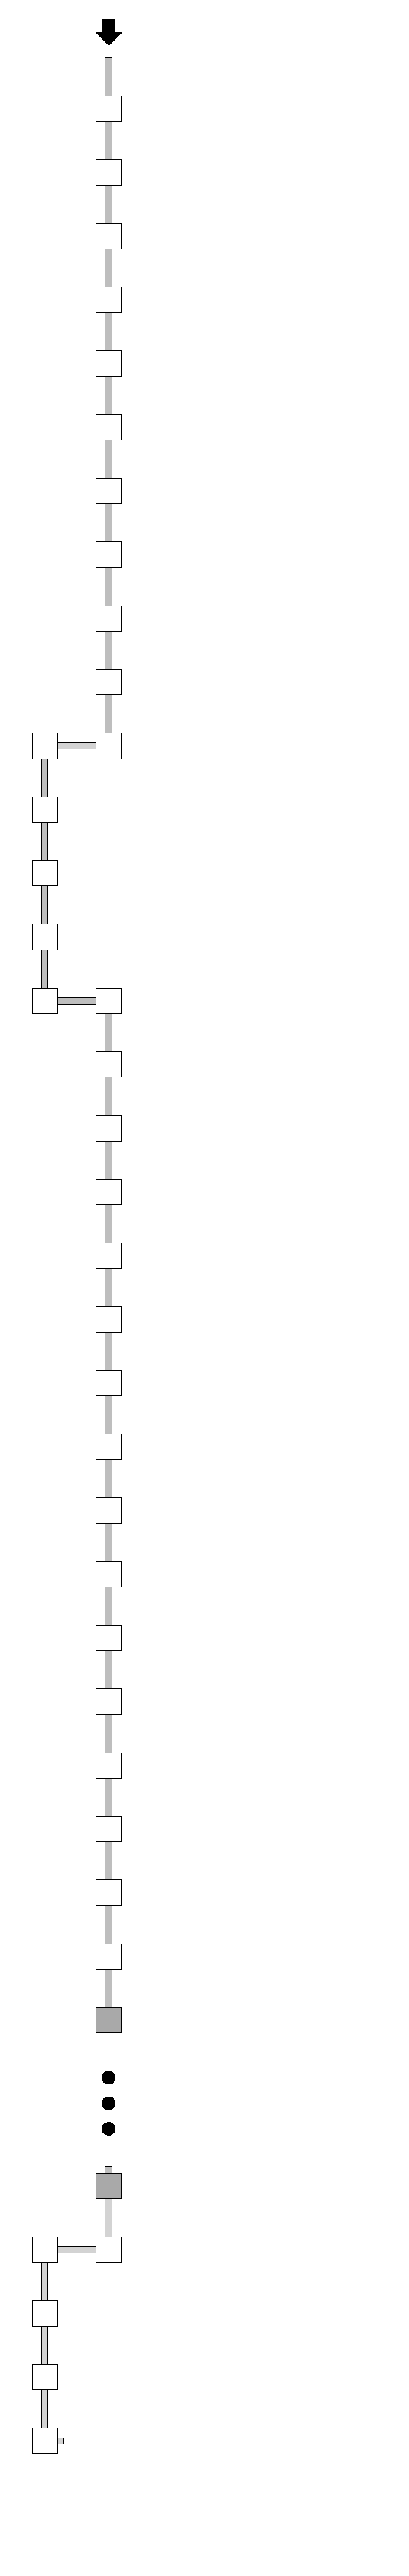
\includegraphics[width=0.45in]{next_read_1-or-2_op_msr_msd}}}%
    ~
    \subcaptionbox{Digit 1 - case 1 overview\label{fig:next_read_1_op_msr_msd_overview}}
    {\makebox[0.24\textwidth][c]{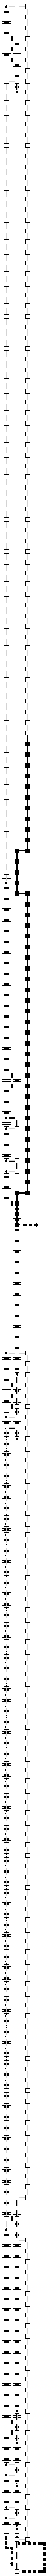
\includegraphics[width=0.45in]{overviews/case1/next_read_1_op_msr_msd}}}%
    ~
\end{figure}

\begin{figure}[H]\ContinuedFloat
    \centering
    \subcaptionbox{Digit 2 - case 2 overview\label{fig:next_read_2_op_msr_msd_overview}}
    {\makebox[0.24\textwidth][c]{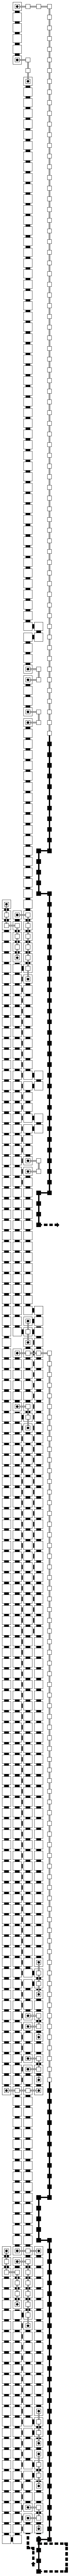
\includegraphics[width=0.45in]{overviews/case2/next_read_2_op_msr_msd}}}%
    ~
    \subcaptionbox{Digit 2 - case 2 (seed) overview\label{fig:next_read_2_seed_op_msr_msd_overview}}
    {\makebox[0.24\textwidth][c]{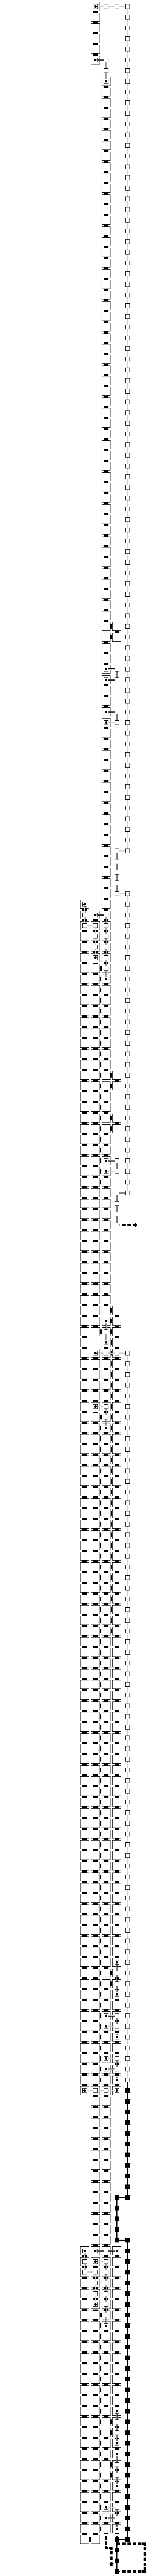
\includegraphics[width=0.45in]{overviews/case2/next_read_2_seed_op_msr_msd}}}%
    ~
    \subcaptionbox{Digit 1 - case 2\label{fig:next_read_1_op_msr}}
    {\makebox[0.24\textwidth][c]{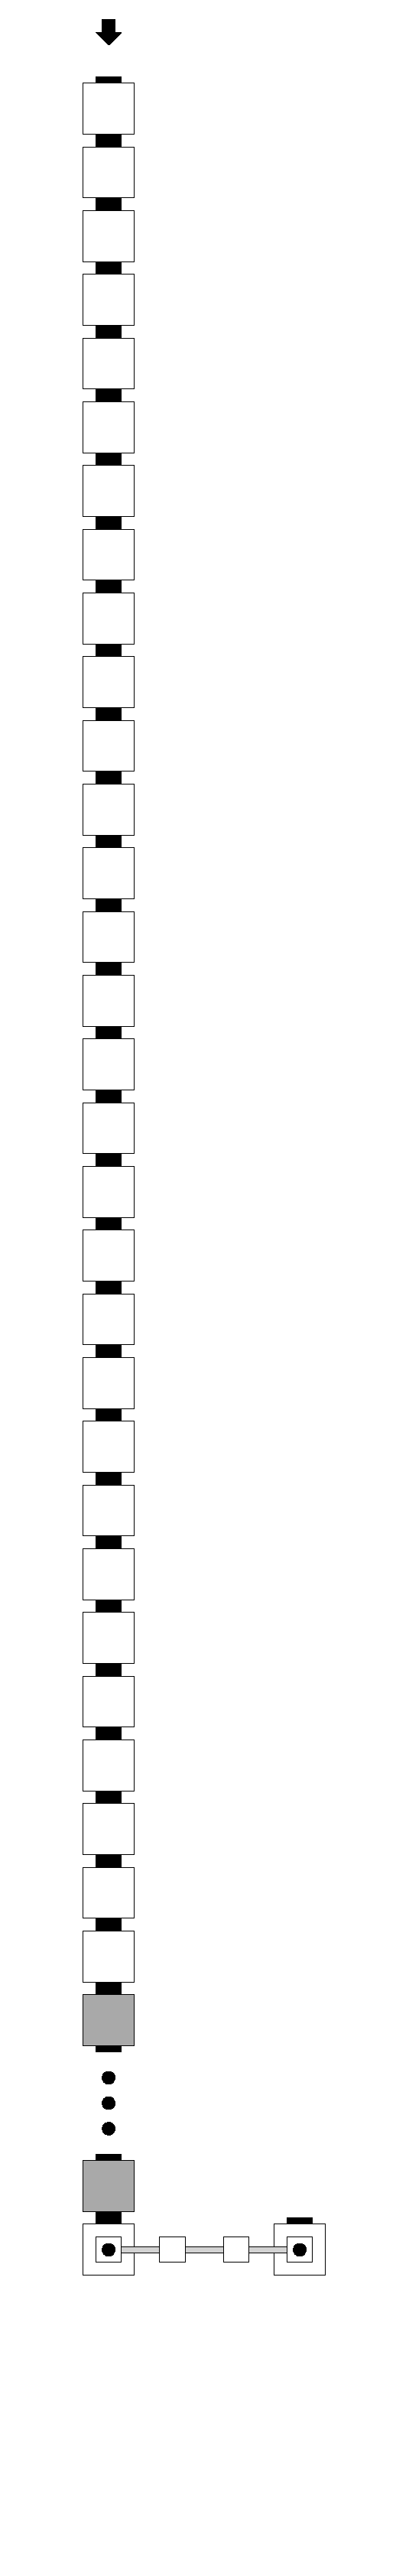
\includegraphics[width=0.45in]{next_read_1_op_msr}}}%
    ~
    \subcaptionbox{Digit 1 - case 2 overview\label{fig:next_read_1_op_msr_overview}}
    {\makebox[0.24\textwidth][c]{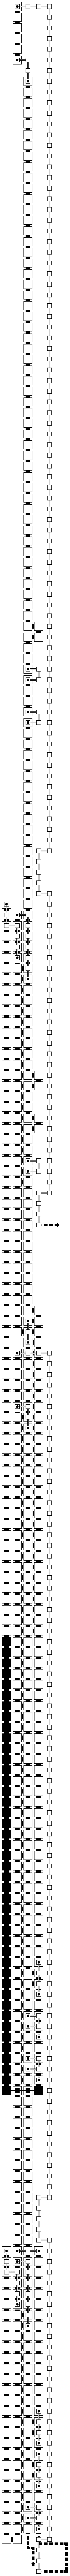
\includegraphics[width=0.45in]{overviews/case2/next_read_1_op_msr}}}%
    ~
\end{figure}

\begin{figure}[H]\ContinuedFloat
    \centering
    \subcaptionbox{Digit 3 - case 3\label{fig:next_read_3_op-or-seed_msr_msd}}
    {\makebox[0.24\textwidth][c]{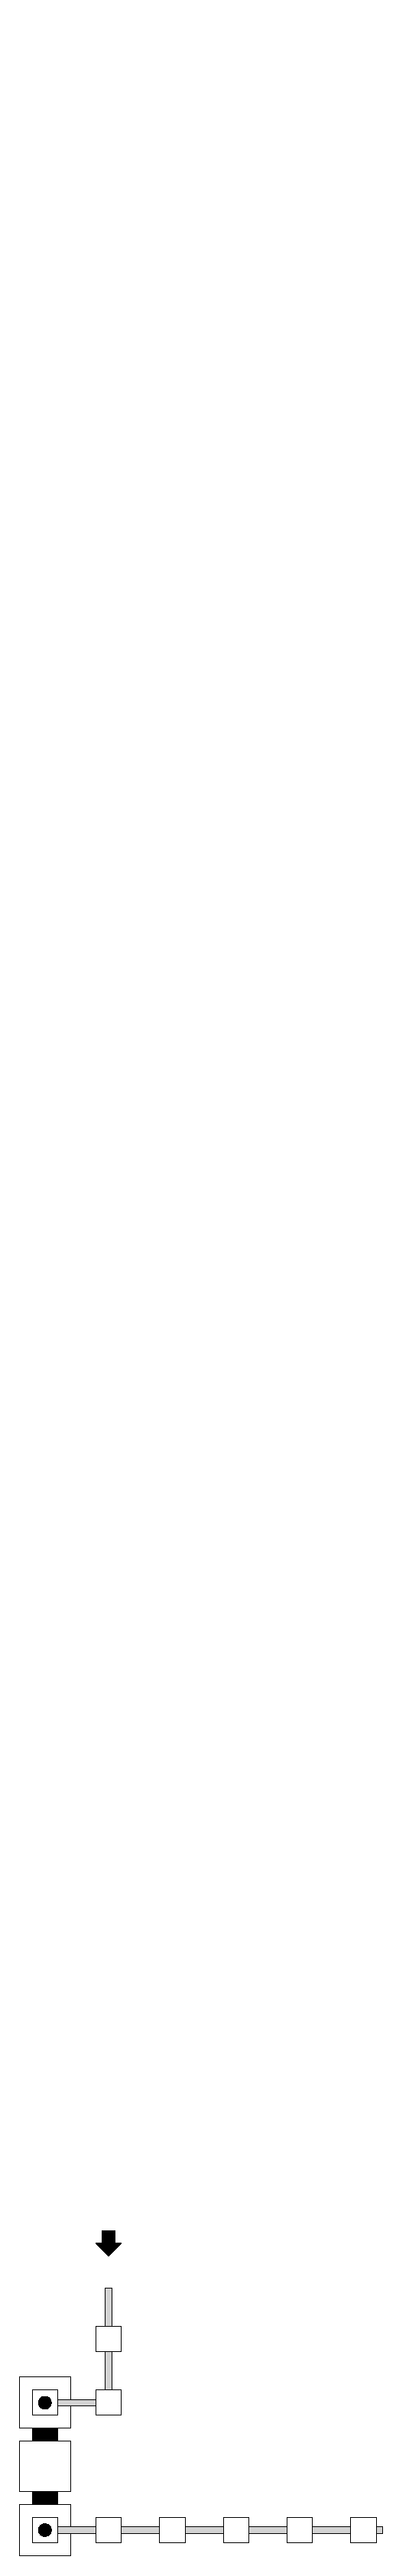
\includegraphics[width=0.45in]{next_read_3_op-or-seed_msr_msd}}}%
    ~
    \subcaptionbox{Digit 3 - case 3 overview\label{fig:next_read_3_op_msr_msd_overview}}
    {\makebox[0.24\textwidth][c]{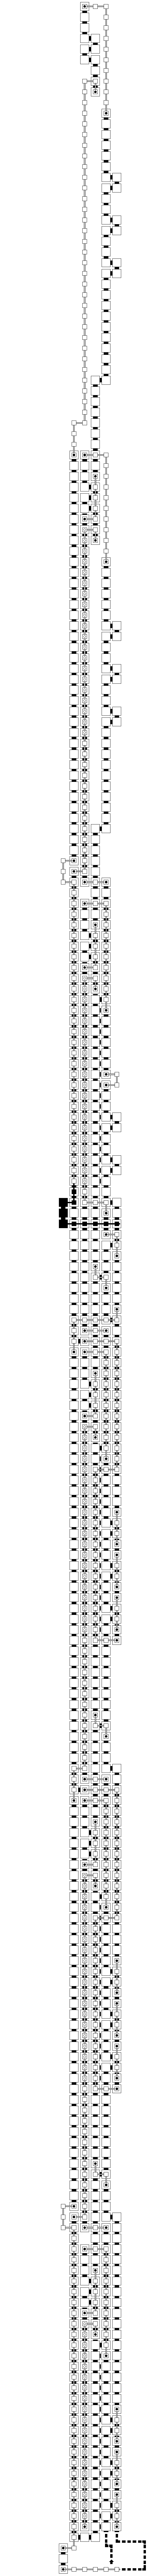
\includegraphics[width=0.45in]{overviews/case3/next_read_3_op_msr_msd}}}%
    ~
    \subcaptionbox{Digit 3 - case 3 (seed) overview\label{fig:next_read_3_seed_op_msr_msd_overview}}
    {\makebox[0.24\textwidth][c]{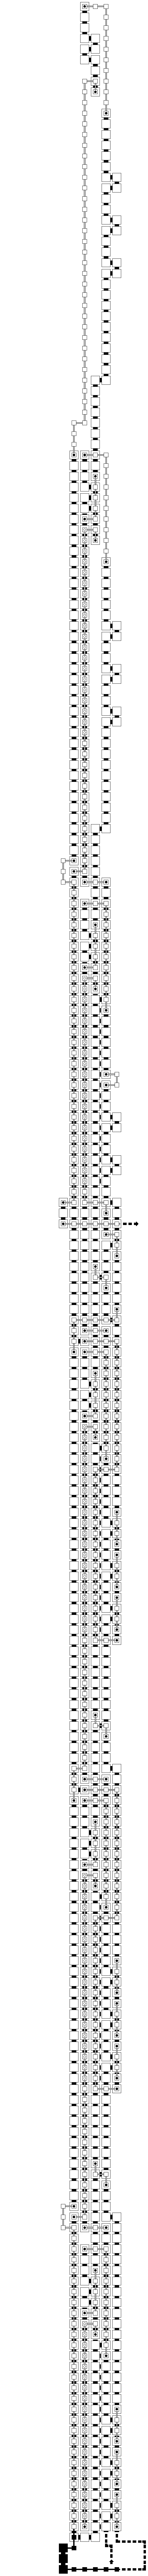
\includegraphics[width=0.45in]{overviews/case3/next_read_3_seed_op_msr_msd}}}%
    ~
    \caption{\label{fig:next_read_gadgets} The {\nextread} gadgets}
\end{figure}


